\scanpage{49}
\inserted{$\Delta_{n+2}(0,1,c_0,\ldots,c_{n-1})$}
\[
\deleted{\unsure{\Delta}}
\Delta_n(\underbrace{c_0,\ldots,c_{n-1}}_{n\ \text{arg.}})
=\unsure{-}\det\left(
\begin{array}{ccccccccc}
0&-1&0&0&0&0&0&\cdots&0\\
-1&2&-c_0&0&0&0&0&\cdots&0\\
0&-c_0&2c_0&-c_1&0&0&0&\cdots&\vdots\\
0&0&-c_1&2c_1&-c_2&-c_3&0&&\vdots\\
0&0&0&&&&&&0\\
\vdots&\vdots&\vdots&&&&&&-c_{n-1}\\
0&0&0&--&0&&&-c_{n-1}&2c_{n-1}
\end{array}\right)
\quad(\text{ordre }n+2)
\]
\[
=\det\left(
\begin{array}{ccccccc}
2c_0&-c_1&0&0&0&\text{---}&0\\
-c_1&2c_1&-c_2&0&0&&\\
0&-c_2&2c_2&-c_3&0&--&\big|\\
0&0&-c_3&2c_3&-c_4&&0\\
--&--&--&--&\text{---}&--&-c_{n-1}\\
0&0&0&0&\cdots&-c_{n-1}&2c_{n-1}
\end{array}\right)
\quad\text{ordre }n
\]
\[
\boxed{\Delta_n(c_0,\ldots,c_{n-1})
=2c_0\Delta_{n-1}(c_1,\ldots,c_{n-1})
\unsure{-}c_1^2\Delta_{\unsure{n-1|n-2}}(c_2,\ldots,c_{n-1})}
\]
\[
\Delta'_n(c_0,\ldots,c_{n-1})=
\begin{cases}
\Delta_n(c_0,\ldots,c_{n-1})&\text{si }n\ \deleted{\unsure{\text{im}}}\text{pair}\\
\frac12\Delta_n(c_0,\ldots,c_{n-1})&\text{si }n\text{ impair}
\end{cases}
\]
Posons
\[
\left.\begin{aligned}
c_0&=\beta_0,\ \unsure{c}\\
c_1&=\beta_0\beta_1\\
&\mathbin{--}\\
c_{n-1}&=\beta_0\beta_1\mathbin{-}\beta_{n-1}
\end{aligned}\right\}
\quad n\ \text{indéterminées }\beta_i
\]
\[
\delta_n(\beta_0,\ldots,\beta_{n-1})
=\Delta_n(\beta_0,\beta_0\beta_1,\ldots,\beta_0\beta_1\mathbin{-}\beta_{n-1})
\]
\[
\delta'_n(\beta_0,\ldots,\beta_{n-1})=\Delta'_n(\ldots)
=\begin{cases}
\delta_n(\beta_0,\mathbin{-}\beta_{n-1})&n\text{ pair}\\
\frac12\delta_n(\beta_0,\mathbin{-}\beta_{n-1})&n\text{ impair}
\end{cases}
\]
\[
\Delta_n,\Delta'_n,\deleted{\unsure{\widetilde\Delta_n}}
\inserted{\widetilde\Delta'_n}\in\mathbb Z[C_0,\ldots,C_{n-1}]
\]
\[
\delta_n,\delta'_n,\widetilde\delta'_n\in\mathbb Z[B_0,\ldots,B_{n-1})
\]
\margin{\[
\begin{aligned}
\Delta'_n[C_0,\mathbin{-},C_{n-1}]
&=C_{n-1}\widetilde\Delta'_{n-1}(C_0,\mathbin{-},C_{n-2})\\
\delta'_n[B_0,\mathbin{-},B_{n-1}]
&=B_{n-1}\widetilde\delta'_n(B_0,\ldots,B_{n-2})
\end{aligned}
\]}
\[
\Delta_1(c_0)=2c_0,\quad\Delta'_1(c_0)=c_0
\qquad\widetilde\Delta'_1(c_0)=1
\]
\[
\Delta_2(c_0,c_1)=4c_0c_1-c_1^2=c_1(4c_0-c_1)
\qquad\widetilde\Delta'_2(c_0,c_1)=4c_0-c_1)
\]
\[
\Delta_3(c_0,c_1,c_2)=2c_2(4c_0c_1-c_0c_2-c_1^2),\quad
\Delta'_3=\deleted{\unsure{2}}c_2(4c_0c_1-c_0c_2-c_1^2),
\]
\[
\mathbin{---}\qquad
\widetilde\Delta'_3(c_0,c_1,c_2)=4c_0c_1-c_0c_2-c_1^2
\]
\[
\Delta_n(C_0,\mathbin{-},C_{n-1})
=\sum_{0\leq p\leq[\frac n2]}(-1)^p2^{n-2p}
\sum_{\substack{\text{suites de }p\\
\deleted{\unsure{\text{intervalles}}}\\
\text{él. de }\unsure{\mathcal P}_2([0,n-1])\\
\text{disjoints}\\
J_1\mathbin{-}J_p,\ \deleted{\unsure{J_i=\{j_i,j_i+1\}}}}}
\prod_{i\in J'}C_i\prod_{j\in J''}C_j^2
\]
\[
J=\bigcup_{1\leq i\leq p}J_i,\qquad
J'=[0,n-1]\setminus J
\]
$J''=$ ens des derniers él'mts des $J_i$
\[
(J''\in\unsure{\mathcal P}_p([0,n-1]))
\]
\margin{\unsure{chgt} notation}
\margin{non, grâce au \unsure{régime} des paires}
\figure{\begin{tikzpicture}
\draw[->] (1.5,1)..controls(1,.5)and(.4,.4)..(0,.2);
\draw (2,1)--(2,.15);
\end{tikzpicture}}
\margin{\uline{NB} Il n'y a pas de cancellation de termes.}

\deleted{$\unsure{\Delta_n(C_0,\ldots,C_{n-1})=}$}
Le monôme $M=\prod_{i\in J'}C_i\prod_{j\in J''}C_j^2$
s'écrit aussi
\[
\deleted{\unsure{\delta_n(c_1,\ldots,c_n)=\beta_0}}
\]
\[
B_0^n B_1^{n-1+\varepsilon_2}
B_{\unsure{3|2}}^{n-2+\varepsilon_3}\mathbin{-}B_{n-1}^{\varepsilon_n}
\]
\[
\varepsilon_k\in\{0,1\}\qquad2\leq k\leq n
\]
\[
\varepsilon_k=1\ \text{sss}\ k\in J'''
\]
(il y en \unsure{a} $p$ tels $k$)
\[
M=\prod_{1\leq i\leq n}C'_i\qquad
C'_i=\begin{cases}
C_i&\text{si }i\in J'\\
C_j&\text{si }j\in J''\\
C_{j+1}&\text{si }j\in\deleted{\unsure{J''}}\inserted{J'''}
\end{cases}
\]
\figure{\begin{tikzpicture}[x=1cm,y=.6cm]
\draw (0,0)--(5,0);
\fill (.15,0) circle (.025);\node[below] at (.15,0){$1$};
\fill (2.3,.08) circle (.025);\node[below] at (2.3,0){$k$};
\fill (4.8,.1) circle (.025);\node[above] at (4.8,.1){$n$};
\end{tikzpicture}}
\[
\delta_n(B_0,\ldots,B_n)
=B_0^nB_1^{n-1}\cdots B_{n-1}^{1}
\underbrace{\unsure{L_n|L_{n-1}}(B_1,\mathbin{-},B_{n-1})}_{
\text{polynôme }\deleted{\text{de degré}}\ \leq[\frac n2]}
\]
\margin{\figure{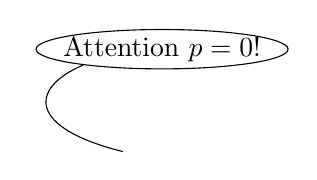
\begin{tikzpicture}
\draw (0,0) ellipse (1.6 and .25);
\node at (0,0){Attention $p=0$!};
\draw (-1,-.2)..controls(-1.7,-.5)and(-1.7,-1)..(-.5,-1.3);
\end{tikzpicture}}}
\deleted{\unsure{Attention!}}
$C'_i$ contient un facteur \uline{$B_k$}
\deleted{\unsure{(et une puissance)}}
(à la puiss. $1$ exactement) sss
\deleted{\unsure{\text{au moins}}}
$i\geq k$, \uline{ou} $i=k-1$ \uline{et}
$i\in J'''$ i.e. $k\in J''$.
\[
\begin{aligned}
\unsure{L_n|L_{n-1}}(B_1,\mathbin{-},B_{n-1})
&=\sum_{0\leq p\leq[\frac n2]}(-1)^p2^{n-2p}
\sum_{\substack{\deleted{\unsure{\text{suite de }p\text{ intervalles}}}\\
\deleted{\unsure{J''}}\ J\in\unsure{\mathcal P}_p([1,n-1])\\
J\ \text{ne contient pas }2\\\text{entiers consécutifs}}}
B_J\\
&=2^n\unsure{-}2^{n-2}\sum_{\unsure{0\leq i\leq n-1}}B_i
+2^{n-4}\sum_{\substack{1\leq i<j\leq n-1\\j\neq i+1}}B_iB_j\\
&\quad-2^{n-6}\sum_{\substack{1\leq i<j<k\leq n\\\unsure{\vdots\quad\vdots}}}
B_iB_jB_k+\cdots
\end{aligned}
\]
\margin{Attention, $n-1$ et non $n$!}
\mspage{48}

